\documentclass[
11pt, % The default document font size, options: 10pt, 11pt, 12pt
codirector, % Uncomment to add a codirector to the title page
]{charter} 

\usepackage{makecell} %
\usepackage{textcomp} %
\usepackage{enumitem}
\usepackage[table]{xcolor}

% El títulos de la memoria, se usa en la carátula y se puede usar el cualquier lugar del documento con el comando \ttitle
\titulo{Sistema de monitoreo remoto de apiarios} 

% Nombre del posgrado, se usa en la carátula y se puede usar el cualquier lugar del documento con el comando \degreename
%\posgrado{Carrera de Especialización en Sistemas Embebidos} 
\posgrado{Carrera de Especialización en Internet de las Cosas} 
%\posgrado{Carrera de Especialización en Intelegencia Artificial}
%\posgrado{Maestría en Sistemas Embebidos} 
%\posgrado{Maestría en Internet de las cosas}

% Tu nombre, se puede usar el cualquier lugar del documento con el comando \authorname
\autor{Lic. Cynthia Escobar} 

% El nombre del director y co-director, se puede usar el cualquier lugar del documento con el comando \supname y \cosupname y \pertesupname y \pertecosupname
\director{Mg. Ing. Carlos Moisés Fontela}
\pertenenciaDirector{FIUBA} 
% FIXME:NO IMPLEMENTADO EL CODIRECTOR ni su pertenencia
\codirector{Esp. Ciro Edgardo Romero} % para que aparezca en la portada se debe descomentar la opción codirector en el documentclass
\pertenenciaCoDirector{FIUBA}

% Nombre del cliente, quien va a aprobar los resultados del proyecto, se puede usar con el comando \clientename y \empclientename
\cliente{Sr. Enrique Soto}
\empresaCliente{La Agroapícola}

% Nombre y pertenencia de los jurados, se pueden usar el cualquier lugar del documento con el comando \jurunoname, \jurdosname y \jurtresname y \perteunoname, \pertedosname y \pertetresname.
\juradoUno{Nombre y Apellido (1)}
\pertenenciaJurUno{pertenencia (1)} 
\juradoDos{Nombre y Apellido (2)}
\pertenenciaJurDos{pertenencia (2)}
\juradoTres{Nombre y Apellido (3)}
\pertenenciaJurTres{pertenencia (3)}
 
\fechaINICIO{21 de octubre de 2021}    %Fecha de inicio de la cursada de GdP \fechaInicioName
\fechaFINALPlan{8 de diciembre de 2021} 	%Fecha de final de cursada de GdP
\fechaFINALTrabajo{20 de noviembre de 2022}	%Fecha de defensa pública del trabajo final


\begin{document}

\maketitle
\thispagestyle{empty}
\pagebreak


\thispagestyle{empty}
{\setlength{\parskip}{0pt}
\tableofcontents{}
}
\pagebreak


\section*{Registros de cambios}
\label{sec:registro}


\begin{table}[ht]
\label{tab:registro}
\centering
\begin{tabularx}{\linewidth}{@{}|c|X|c|@{}}
\hline
\rowcolor[HTML]{C0C0C0} 
Revisión & \multicolumn{1}{c|}{\cellcolor[HTML]{C0C0C0}Detalles de los cambios realizados} & Fecha      \\ \hline
0      & Creación del documento                                 & 21/10/2021 \\ \hline
1      & Se completa hasta el punto 5 inclusive                 & 01/11/2021 \\ \hline
2      & Se completa hasta el punto 9 inclusive                 & 08/11/2021 \\ \hline
3      & Se completa hasta el punto 11 inclusive                 & 17/11/2021 \\ \hline
4      & Se completa el plan & 25/11/2021 \\ \hline
\end{tabularx}
\end{table}

\pagebreak



\section*{Acta de constitución del proyecto}
\label{sec:acta}

\begin{flushright}
Buenos Aires, \fechaInicioName
\end{flushright}

\vspace{2cm}

Por medio de la presente se acuerda con la \authorname\hspace{1px} que su Trabajo Final de la \degreename\hspace{1px} se titulará ``\ttitle''. Consistirá esencialmente en el prototipo preliminar de un sistema de medición, visualización y emisión de alertas destinado al monitoreo de apiarios, y tendrá un presupuesto preliminar estimado de 600 hs de trabajo y {\$250000}, con fecha de inicio \fechaInicioName\hspace{1px} y fecha de presentación pública \fechaFinalName.

%50k + 250 $/h * cant horas humanas + 50k (por gastos extras) = 250k

Se adjunta a esta acta la planificación inicial.

\vfill

% Esta parte se construye sola con la información que hayan cargado en el preámbulo del documento y no debe modificarla
\begin{table}[ht]
\centering
\begin{tabular}{ccc}
\begin{tabular}[c]{@{}c@{}}Ariel Lutenberg \\ Director posgrado FIUBA\end{tabular} & \hspace{2cm} & \begin{tabular}[c]{@{}c@{}}\clientename \\ \empclientename \end{tabular} \vspace{2.5cm} \\ 
\multicolumn{3}{c}{\begin{tabular}[c]{@{}c@{}} \supname \\ Director del Trabajo Final\end{tabular}} \vspace{2.5cm} \\
%\begin{tabular}[c]{@{}c@{}}\jurunoname \\ Jurado del Trabajo Final\end{tabular}     &  & \begin{tabular}[c]{@{}c@{}}\jurdosname\\ Jurado del Trabajo Final\end{tabular}  \vspace{2.5cm}  \\
%\multicolumn{3}{c}{\begin{tabular}[c]{@{}c@{}} \jurtresname\\ Jurado del Trabajo Final\end{tabular}} \vspace{.5cm}                                                                     
\end{tabular}
\end{table}




\section{1. Descripción técnica-conceptual del proyecto a realizar}
\label{sec:descripcion}

Las abejas son indispensables en la conservación del ecosistema y en la producción de alimentos gracias al importante papel que juegan como polinizadores en la fertilización y reproducción de las plantas.
% ya que en su afán de alimentarse transportan polen de flor en flor y contribuyen a la fecundación y reproducción de las plantas.

La apicultura es la actividad realizada por el hombre que consiste en la cría y en el cuidado apropiado de las abejas para lograr que sus colonias prosperen y se pueda obtener de ellas para el consumo y/o comercialización: miel, polen, jalea real, propóleo y cera.

Es una actividad noble que a pesar de tener un fin económico trabaja buscando un equilibrio entre la explotación comercial y preservación de las abejas y el medio ambiente.

A pesar de los avances tecnológicos la apicultura sigue siendo una práctica casi artesana ya que el apicultor debe estar muy involucrado en el mantenimiento y cuidado de sus colmenas. Se deben realizar visitas periódicas para controlar la salubridad de las abejas, chequear los niveles de alimentos y el estado general de las colmenas.
Como los apiarios suelen estar instalados lejos de los centros urbanos estas visitas suelen consumir tiempo y recursos, y de no realizar visitas periódicas uno se arriesga a poder perder colmenas.

El objetivo de esta solución es ayudar a minimizar la intervención del apicultor y sus costos asociados al proveerle de una herramienta que le permita monitorear distintas variables de sus colmenas de manera remota.


El monitoreo remoto propuesto se planea realizar a través de la recopilación de datos con los siguientes instrumentos instalados dentro de la cámara de cría de una colmena de abejas europeas (\textit{Apis mellifera}):
\begin{itemize}
\item Sensor de temperatura. 
\item Sensor de humedad.
\item Sensor de sonido.
\item Sensor de inclinación (giróscopo).
\end{itemize}


En la figura 1 se presenta el diagrama en bloques del sistema que representa los distintos componentes que trabajarán en conjunto para recopilar datos y permitir controlar remotamente el estado de las colmenas.

\begin{figure}[htpb]
\centering 
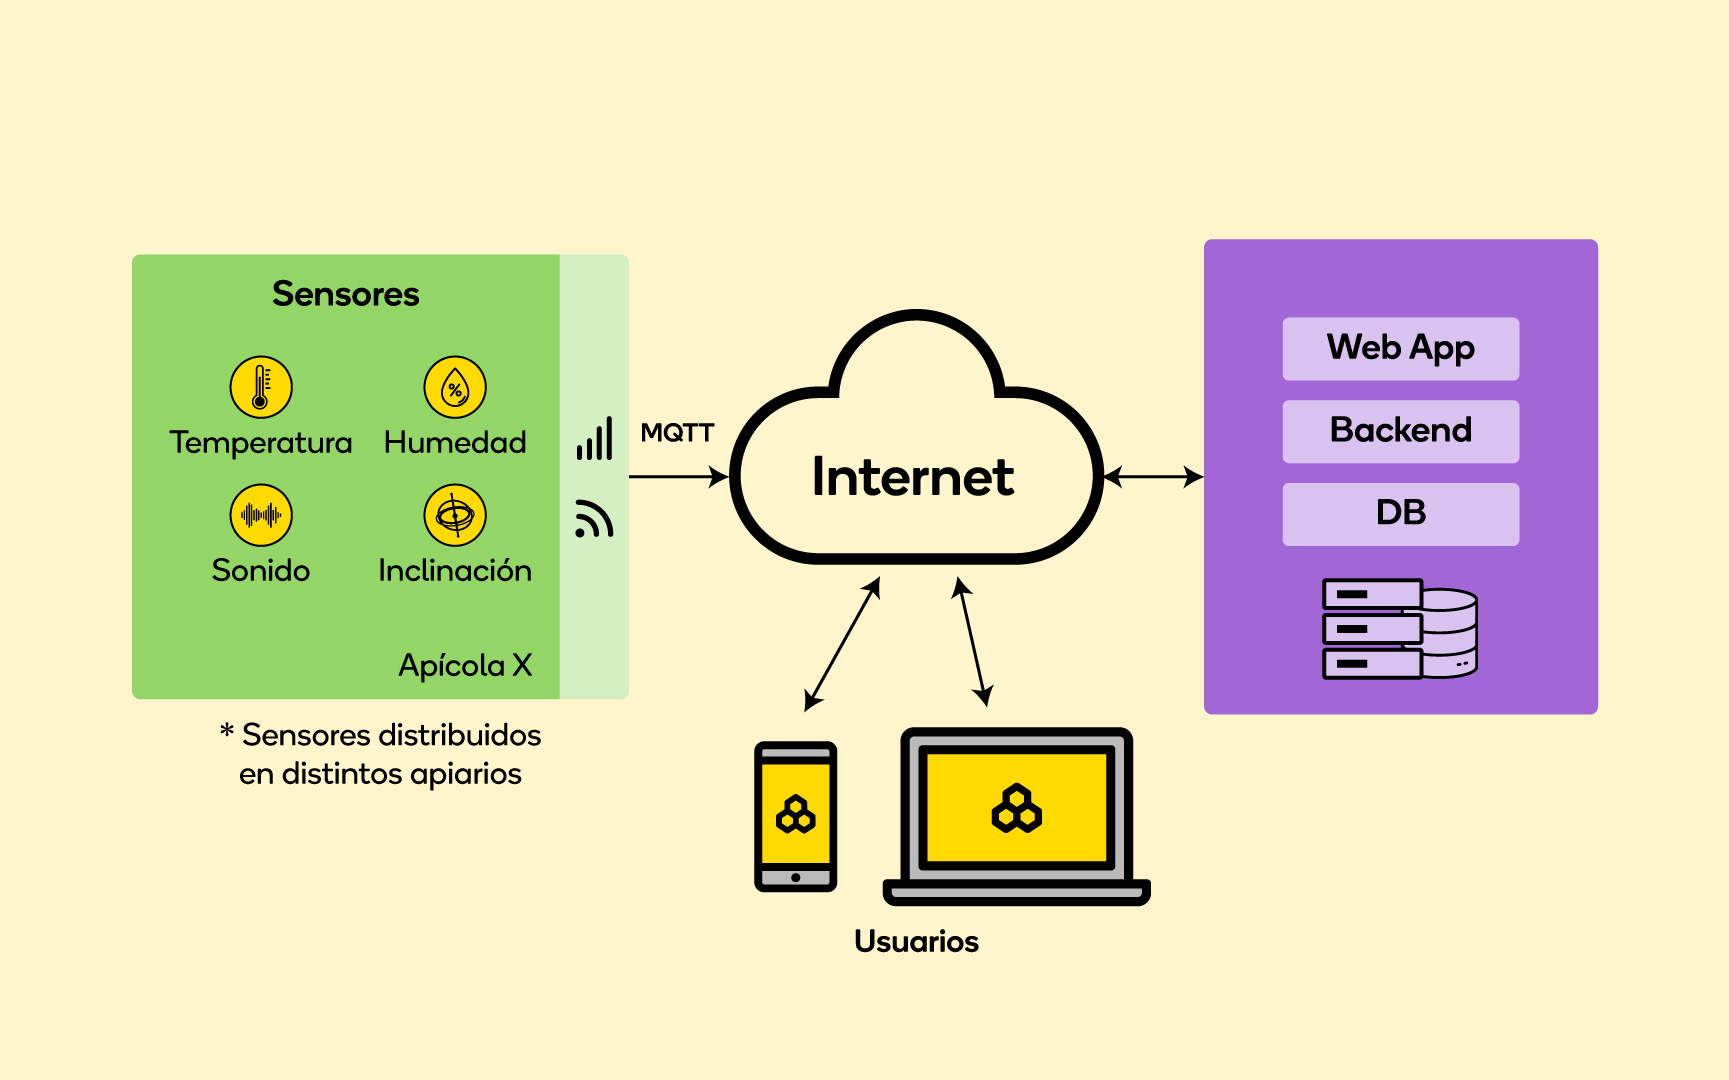
\includegraphics[width=1\textwidth]{./Figuras/diagBloquesPropio.jpg}
\caption{Diagrama en bloques del sistema.}
\label{fig:diagBloques}
\end{figure}



La solución se compone de las siguientes partes:
\begin{itemize}
\item Medición de la temperatura, de la humedad y del sonido en el interior de la cámara de cría y de su inclinación.
%\item transporte de los datos
\item Lógica de procesamiento y persistencia de datos.
\item Visualización de métricas y alarmas.
\end{itemize}

Se propone que las mediciones sean recolectadas en los apiarios, transmitidas a un broker MQTT para finalmente ser enviadas a un servicio backend para su procesamiento, análisis y persistencia.
También se contempla el desarrollo de un frontend para que el usuario pueda:
\begin{itemize}
\item Acceder a la visualización de las métricas y alertas.
\item Acceder a un dashboard de administración y configuración.
\end{itemize}
Desde este frontend se espera que el usuario pueda establecer los thresholds de aceptabilidad para cada una de las métricas, así como la configuración de las acciones a tomar luego del disparo de una alarma de sistema.

%\vspace{25px}
\section{2. Identificación y análisis de los interesados}
\label{sec:interesados}

\begin{table}[ht]
%\caption{Identificación de los interesados}
%\label{tab:interesados}
\begin{tabularx}{\columnwidth}{@{}|l|X|l|l|@{}}
\hline
\rowcolor[HTML]{C0C0C0} 
Rol           & Nombre y Apellido & Organización 	& Puesto 	\\ \hline
%Auspiciante   &        -          &        -      	&     -   	\\ \hline
Cliente       & \clientename      &\empclientename	&    -   	\\ \hline
%Impulsor      &                   &              	&        	\\ \hline
Responsable   & \authorname       & FIUBA        	& Alumno 	\\ \hline
Colaboradores &      Sr. Anibal Taverna             & MAGyP            	&     Coordinación de Apicultura   	\\ \hline
Orientadores  & \makecell[l]{Mg. Ing. Carlos M. Fontela \\ \cosupname}	       & \pertesupname 	& \makecell[l]{Director Trabajo final\\Codirector Trabajo final} \\ \hline
%Equipo        & -  &  - & - \\ \hline
%Opositores    &                   &              	&        	\\ \hline
Usuario final & Apicultores               &       -       	&     -   	\\ \hline
\end{tabularx}
\end{table}

\begin{itemize}
\item Cliente: es quien dará la aprobación del producto si las pruebas demuestran una mejora en la actividad.
\item Responsable: es quien estará a cargo del análisis, planificación y desarrollo del proyecto.
\item Colaborador: se trata de una autoridad en la actividad que es fuente de información y consejo tanto en lo técnico como en lo práctico.
\item Orientador: es quien en base a su extensa experiencia colaborará en la revisión y planificación del proyecto, y será una guía de referencia para el responsable.
\item Usuario Final: es aquella persona cuya actividad es la apicultura y que se beneficiará del desarrollo de este proyecto.
\end{itemize}

\section{3. Propósito del proyecto}
\label{sec:proposito}

El propósito de este proyecto es colaborar con el cuidado de las colonias de abejas a cargo de apicultores y mejorar la productividad de la actividad poniendo en marcha un sistema que recabe información de las condiciones internas de la cámara de cría. De esta forma permite detectar de manera temprana enfermedades, accidentes y enjambrazones (abandono de la reina de la colmena para crear una nueva colonia)  minimizando la pérdida de colmenas con una intervención mínima del apicultor.

\section{4. Alcance del proyecto}
\label{sec:alcance}

El alcance de este proyecto incluye: 
\begin{itemize}
\item Desarrollo de una aplicación backend que se encargue de:
	\begin{itemize}
	\item Gestión de usuarios, configuraciones de thresholds, alertas y notificaciones.
	\item Procesamiento de las mediciones capturadas.
	\item Gestión de altas, bajas y modificaciones de nuevos apiarios.
	\end{itemize}
\item Desarrollo de una aplicación web que permita visualizar las métricas y acceder a la configuración del sistema.
\item Desarrollo de un prototipo que integre los sensores instalados en el interior de la cámara de cría, con capacidad de conectarse a internet para el envío de los datos a un servidor.
\end{itemize}

El presente proyecto no incluye:

\begin{itemize}
\item La confección de la placa PCB.
\item Instalación de red WiFi.
\item Instalación y configuración de un servidor y la base de datos asociada.
\end{itemize}

\section{5. Supuestos del proyecto}
\label{sec:supuestos}

Para el desarrollo del presente proyecto se supone que:

\begin{itemize}
\item Se tendrá acceso a una red WiFi o a la red GSM/GPRS en el apiario.
\item Se simularán los sensores con distintas configuraciones ambientales.
\item Se contará con la colaboración del cliente para la evaluación de las pruebas.
\item Se contará con el tiempo suficiente para realizar las distintas tareas.
\item Se dispondrá de una colmena de abejas europeas para realizar pruebas.
\item El dispositivo que vivirá dentro de la colmena podrá transmitir información a pesar de ser propolizado.
\item La presencia del dispositivo no impactará en la rutina de la colonia ni del apicultor.
\end{itemize}

\section{6. Requerimientos}
\label{sec:requerimientos}

%Los requerimientos deben numerarse y de ser posible estar agruparlos por afinidad, por ejemplo:

\begin{enumerate}
	\item Requerimientos del nodo de medición:
		\begin{enumerate}
			\item Deberá estar protegido para evitar que las abejas recubran su superficie con propóleo (propolización) que pueda afectar su funcionamiento.
			\item Deberá medir la temperatura en un rago de 0 \textdegree{}C--50 \textdegree{}C.
			\item Deberá medir la humedad en un rango de 0--100\%.
			\item Deberá medir el sonido en un rango de 100 Hz--10kHz.
			\item Deberá medir la posición haciendo uso de un giroscopio y un acelerómetro.
			\item Deberá realizar las capturas cada 3 minutos.
			\item Deberá contar con tecnología GSM/GPRS para la conexión a la red de datos.
			\item Deberá tener un identificador unívoco.
			\item Deberá conectarse a un servidor externo para obtener la hora.
			\item Deberá sincronizar el reloj interno para que independientemente de la hora de impacto en el backend la hora de medición sea confiable.
			\item Deberá contar con almacenamiento local (MicroSD).
			\item Deberá tener capacidad para reintentar el envío de métricas ante pérdida de conexión.
		\end{enumerate}
	\item Requerimientos de seguridad:
		\begin{enumerate}
			\item Autenticación de los nodos y encriptación de los datos utilizando Mutual TLS.
			\item Acceso a la aplicación web con usuario y contraseña.
		\end{enumerate}
	\item Requerimientos de la aplicación backend:
		\begin{enumerate}
			\item Deberá enviar un alerta al usuario cuando detecte que la posición vertical de la colmena ha variado.
			\item Deberá enviar un alerta al detectar que la temperatura en la cámara de cría varía por fuera de los 34\textdegree{}C--36\textdegree{}C.
			\item Deberá enviar un alerta al usuario cuando detecte un cambio brusco de la temperatura en la cámara de cría.
			\item Deberá emitir un alerta cuando se detecte que la humedad ha superado el 14\%.
			\item Deberá mantener un histórico de las métricas de hasta 2 años para comparar resultados de distintas temporadas.
		\end{enumerate}
	\item Requerimientos de la aplicación web:
		\begin{enumerate}		
			\item Deberá mostrar la temperatura en una serie temporal.
			\item Deberá mostrar la humedad en una serie temporal.
			\item Deberá mostrar el sonido en una serie temporal.	
			\item Deberá mostrar la posicion en una serie temporal.
			\item Deberá mostrar la configuración personal del usuario.
			\item Deberá mostrar un histórico de los alertas.
		\end{enumerate}
	\item Requerimientos de documentación del trabajo:
		\begin{enumerate}
			\item Se debe generar un documento de casos de prueba.
			\item Se debe generar un manual de usuario.
		\end{enumerate}	
\end{enumerate}


\section{7. Historias de usuarios (\textit{Product backlog})}
\label{sec:backlog}

Para la ponderación de las historias de usuario descriptas en esta sección se eligió una escala basada en la serie Fibonacci y se tendrá en cuenta la dificultad y complejidad en resolverlas:

\begin{tabular}{|c|c|}
\hline
\rowcolor[HTML]{C0C0C0} 
Dificultad & Ponderación \\ \hline
Baja      & 1 \\ \hline
Media      & 3 \\ \hline
Alta      & 5 \\ \hline
\end{tabular}

\begin{tabular}{|c|c|}
\hline
\rowcolor[HTML]{C0C0C0} 
Complejidad & Ponderación \\ \hline
Baja      & 1 \\ \hline
Media      & 5 \\ \hline
Alta      & 8 \\ \hline
\end{tabular}

\begin{tabular}{|c|c|c|}
\hline
\rowcolor[HTML]{C0C0C0} 
Dificultad & Complejidad & Story Points \\ \hline
1 & 1 & 3 \\ \hline
1 & 5 & 5 \\ \hline
1 & 8 & 8 \\ \hline
3 & 1 & 5 \\ \hline
3 & 5 & 8 \\ \hline
3 & 8 & 13 \\ \hline
5 & 1 & 5 \\ \hline
5 & 5 & 8 \\ \hline
5 & 8 & 13 \\ \hline
\end{tabular}

A continuación se presentan las historias de usuarios:
\begin{itemize}
	\item Como usuario quiero acceder a la aplicación web con mi correo y contraseña para poder verificar el estado de mis colmenas. Dificultad: 5. Complejidad: 8. SP: 13.
	\item Como usuario quiero modificar mi configuración. Dificultad: 5. Complejidad: 3. SP: 8.
	\item Como apicultor quiero poder visualizar la temperatura de cualquiera de mis colmenas. Dificultad: 3. Complejidad: 5. SP: 8.
	\item Como apicultor quiero poder recibir un alerta si la temperatura fluctúa fuera de los 34\textdegree{}C--36\textdegree{}C. Dificultad: 1. Complejidad: 5. SP: 5.
	\item Como apicultor quiero poder visualizar la humedad de cualquiera de mis colmenas. Dificultad: 3. Complejidad: 5. SP: 8.
	\item Como apicultor quiero poder recibir un alerta si la humedad fluctúa por sobre el 14 \%. Dificultad: 1. Complejidad: 5. SP: 5.
	\item Como apicultor quiero poder visualizar la posición de cualquiera de mis colmenas. Dificultad: 3. Complejidad: 5. SP: 8.
	\item Como apicultor quiero poder recibir un alerta si la posición vertical de la colmena ha variado. Dificultad: 1. Complejidad: 5. SP: 5.
	\item Como apicultor quiero poder acceder al histórico de alertas. Dificultad: 3. Complejidad: 5. SP: 8.
	\item Como investigador quiero poder acceder al histórico de cualquiera de las métricas. Dificultad: 5. Complejidad: 5. SP: 8.
\end{itemize}

\section{8. Entregables principales del proyecto}
\label{sec:entregables}

Los entregables del proyecto son:

\begin{itemize}
	\item Manual de usuario.
	\item Diagrama esquemático de la solución.
	\item Prototipo funcional.
	\item Informes de avance y final del proyecto.
	\item Presentación del proyecto.
\end{itemize}

\section{9. Desglose del trabajo en tareas}
\label{sec:wbs}

\begin{enumerate}
\item Planificación general (50 hs):
	\begin{enumerate}
	\item Investigación previa sobre la actividad (20 hs).
	\item Búsqueda de colaboradores y clientes (10 hs).
	\item Charlas informativas con colaboradores (10 hs).
	\item Definición de alcances y requerimientos (10 hs).
	\end{enumerate}
\item Aplicación backend (110 hs):
	\begin{enumerate}
	\item Diseño de modelo de datos (10 hs).
	\item Creación de certificados (10 hs).
	\item Diseño y construcción de la aplicación (50 hs).
	\item Pruebas unitarias (30 hs).
	\item Pruebas de integración (10 hs).
	\end{enumerate}
\item Aplicación web (103 hs):
	\begin{enumerate}
	\item Maquetado (12 hs).
	\item Visualización de métricas (20 hs).
	\item Visualización de alertas (20 hs).
	\item Gestión de configuración (15 hs).
	\item Gestión de usuarios (10 hs).
	\item Pruebas de visualización de métricas (8 hs).
	\item Pruebas de visualización de alertas (8 hs).
	\item Pruebas de integración (10 hs).
	\end{enumerate}
\item Desarrollo del prototipo (53 hs):
	\begin{enumerate}
		\item Análisis y selección de sensor de temperatura (3 hs).
		\item Análisis y selección de sensor de humedad (3 hs).
		\item Análisis y selección de sensor de sonido (4 hs).
		\item Análisis y selección de sensor de posición (3 hs).	
		\item Investigación sobre microcontroladores disponibles (10 hs).
		\item Integración de componentes (20 hs).		
		\item Instalación y protección de nodo de sensores (10 hs).
	\end{enumerate}
\item Firmware del prototipo (179 hs):
	\begin{enumerate}
		\item Diseño de arquitectura (12 hs).
		\item Programación de giroscopio y acelerómetro (15 hs).		
		\item Estudio y programación del módulo GSM/GPRS (30 hs).
		\item Programación de la sincronización del reloj interno (5 hs).
		\item Estudio de Mutual TLS y creación de certificados (12 hs).
		\item Manipulación de datos (25 hs).
		\item Desarrollo de la comunicación utilizando Mutual TLS (35 hs).
		\item Pruebas unitarias (30 hs)
		\item Prubas de integración (15 hs).
	\end{enumerate}
\item Documentación (95 hs):
	\begin{enumerate}
		\item Elaboración de manual de pruebas (10 hs).
		\item Elaboración de manual de usuario (15 hs).
		\item Elaboración del informe de avance (30 hs).		
		\item Elaboración de la memoria técnica (40 hs).
	\end{enumerate}
\item Cierre (50 hs):
	\begin{enumerate}
		\item Elaboración del informe final (30 hs).	
		\item Elaboración de la presentación (20 hs).
	\end{enumerate}
\end{enumerate}

Cantidad total de horas: (640 hs)

\section{10. Diagrama de Activity On Node}
\label{sec:AoN}

En el diagrama de actividades se puede observar en rojo el camino crítico y la unidad de tiempo (t) está expresada en horas.

\begin{figure}[htpb]
\centering 
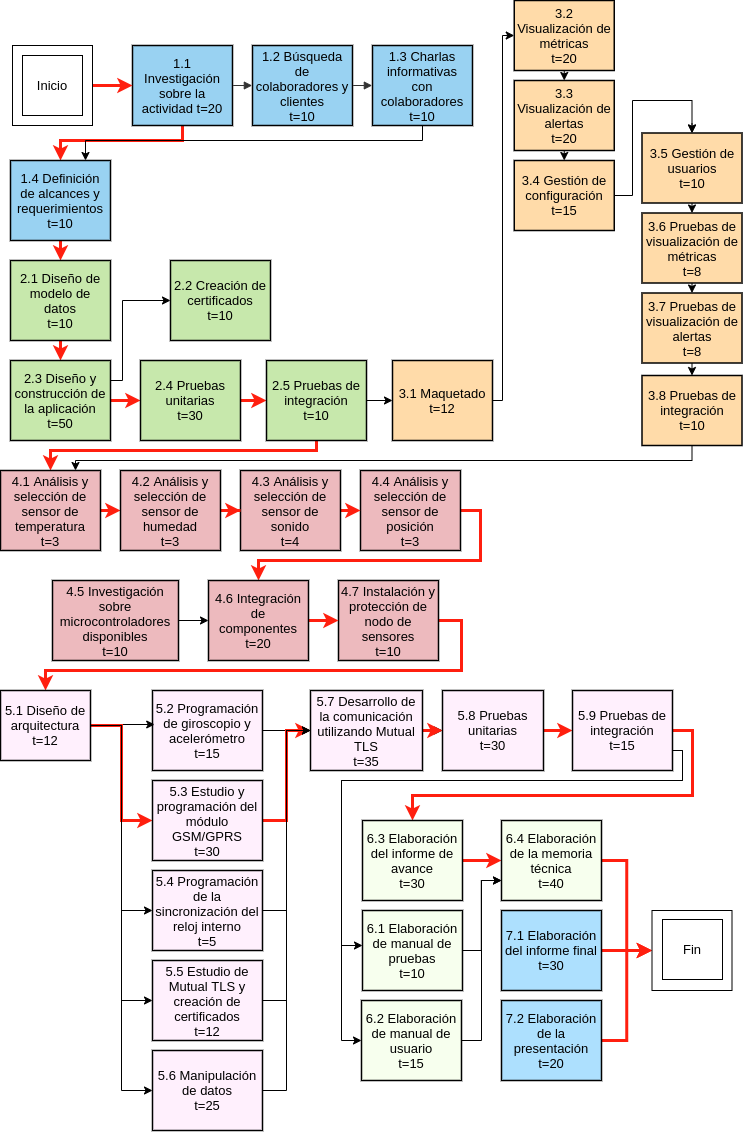
\includegraphics[width=1\textwidth]{./Figuras/Activity-on-node-v4.png}
\caption{Diagrama en \textit{Activity on Node}.}
\label{fig:AoN}
\end{figure}

\begin{figure}[htpb]
\centering 
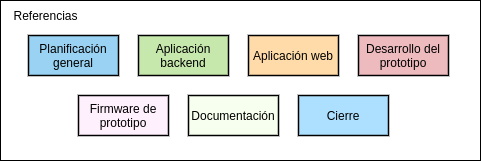
\includegraphics[width=0.8\textwidth]{./Figuras/Ref-Activity-on-node.png}
\caption{Referencias del diagrama en \textit{Activity on Node}.}
\label{fig:Ref_fordAoN}
\end{figure}


\section{11. Diagrama de Gantt}
\label{sec:gantt}

En el siguiente diagrama de Gantt se considera que sólo se dispondrá de un recurso 3 hs al día.

\begin{figure}[htpb]
\centering 
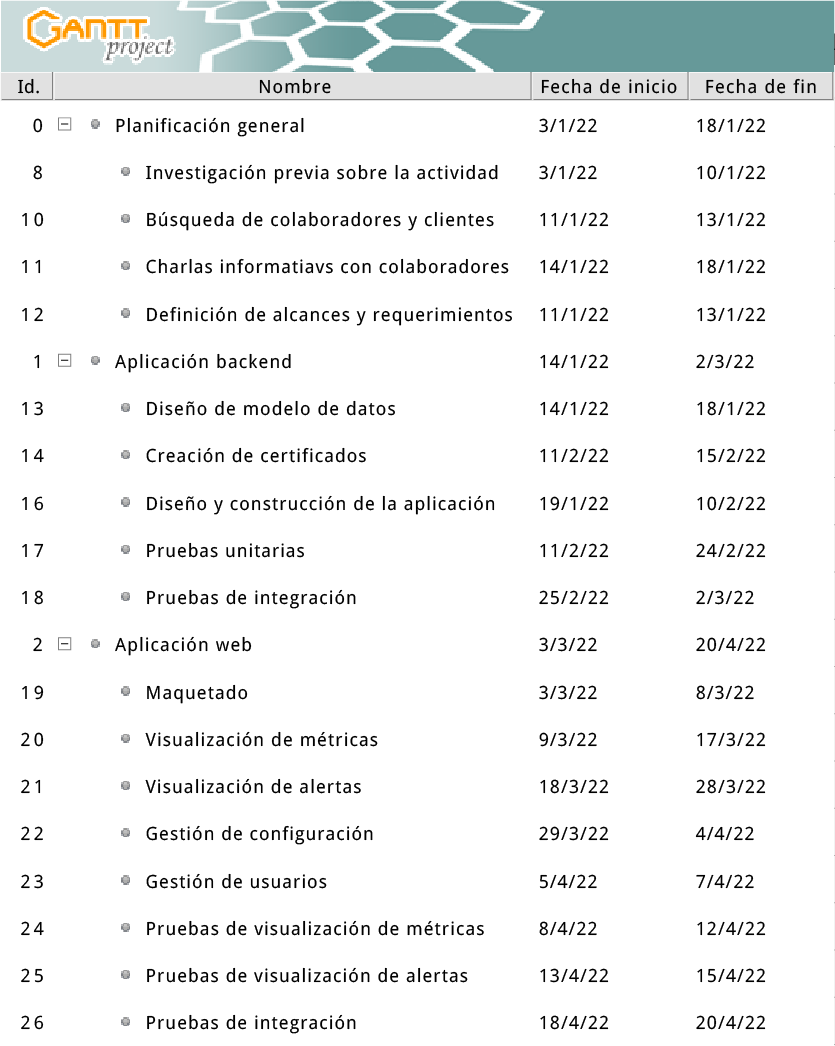
\includegraphics[width=.8\textwidth]{./Figuras/gantt-1.png}
\caption{Diagrama Gantt parte 1 de 4.}
\label{fig:gantt1}
\end{figure}

\begin{figure}[htpb]
\centering 
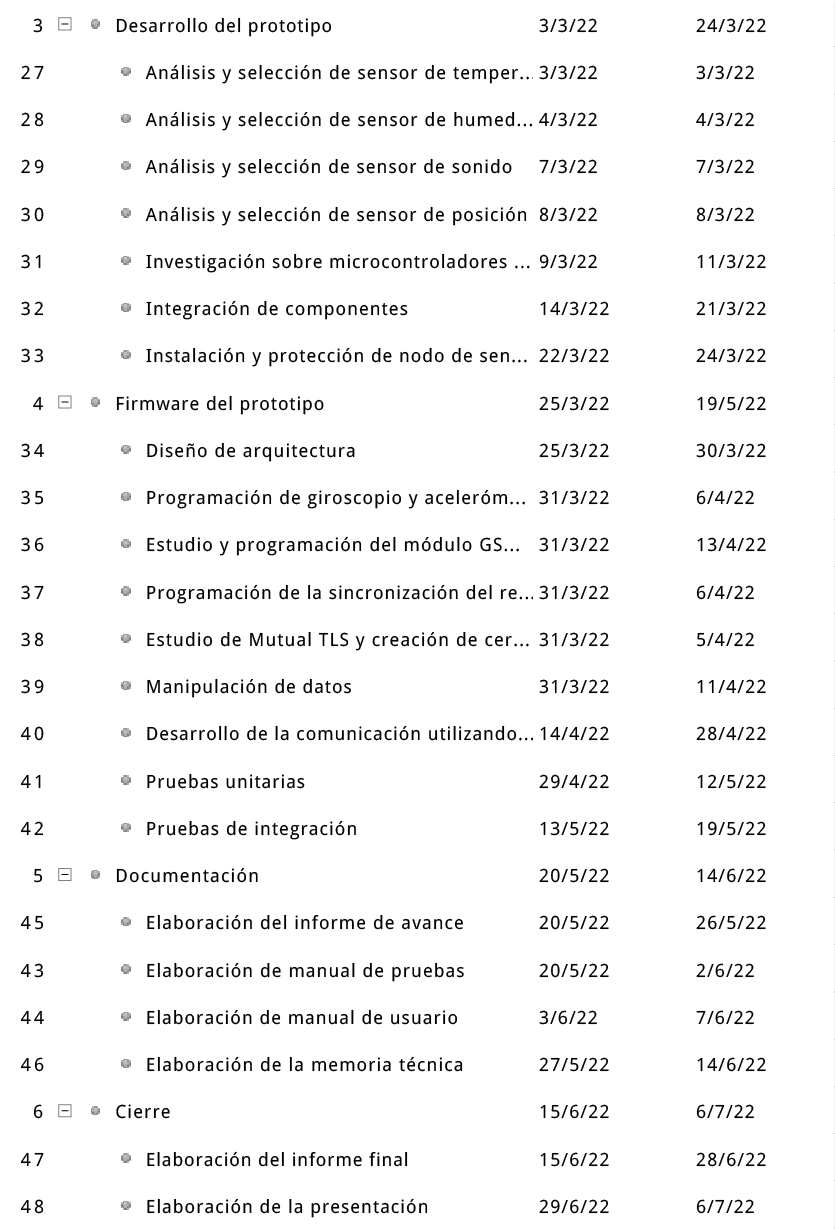
\includegraphics[width=.8\textwidth]{./Figuras/gantt-2.png}
\caption{Diagrama Gantt parte 2 de 4.}
\label{fig:gantt2}
\end{figure}

\begin{figure}[htpb]
\centering 
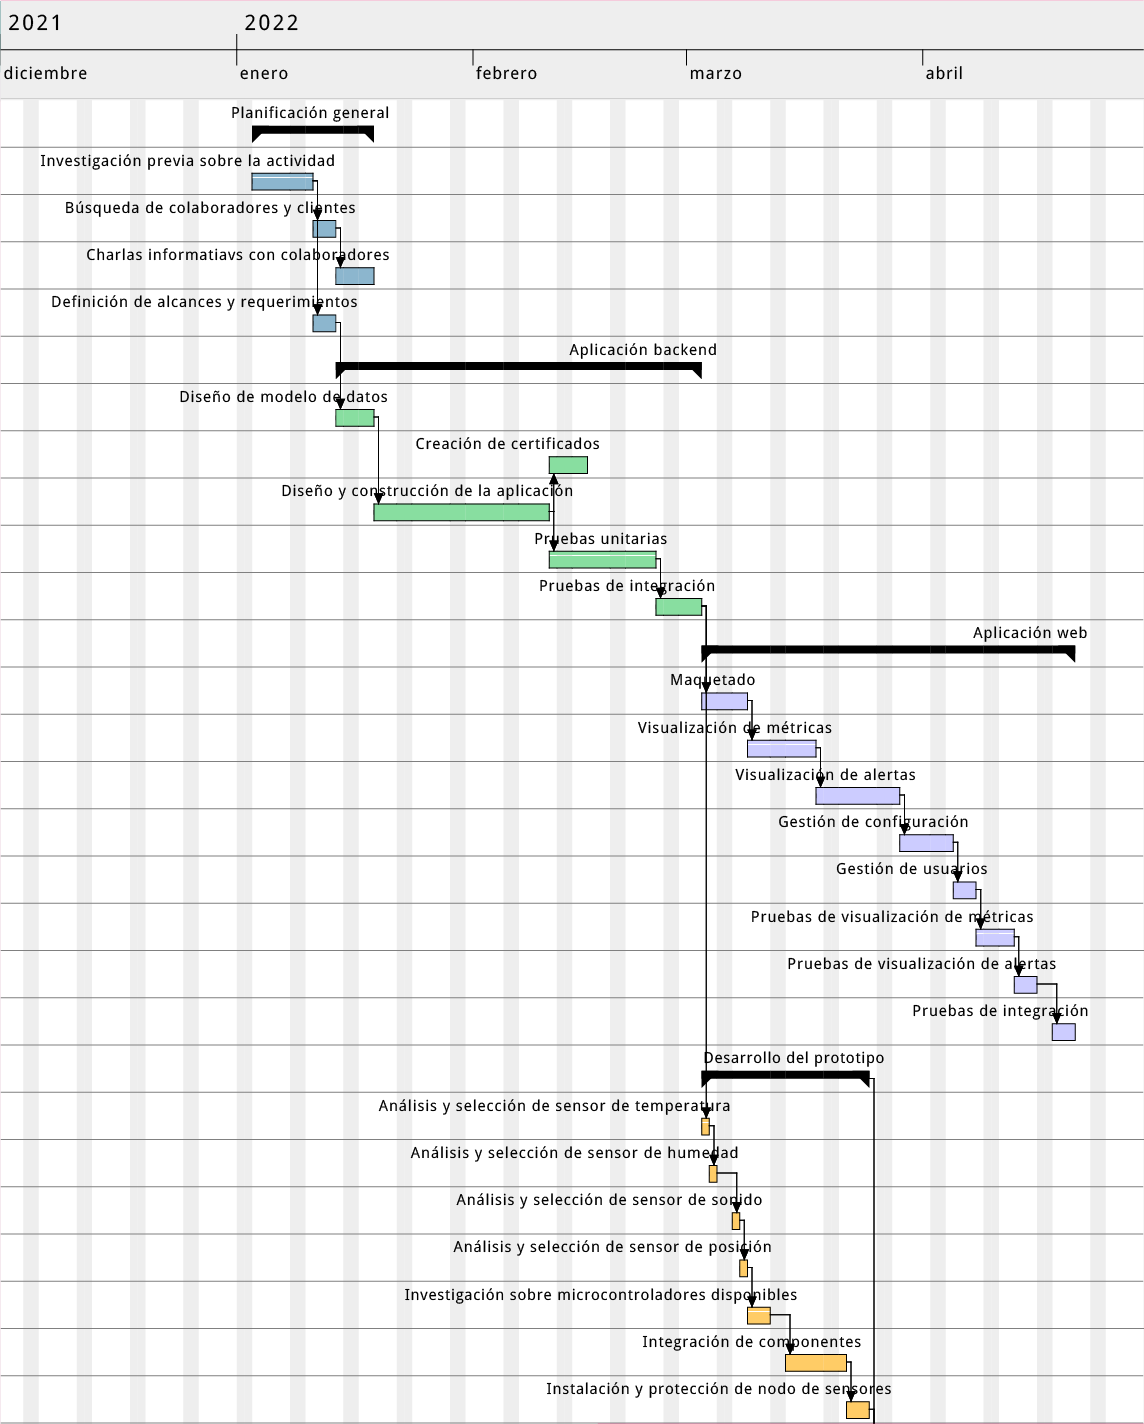
\includegraphics[width=1.1\textwidth]{./Figuras/gantt-3-bis.png}
\caption{Diagrama Gantt parte 3 de 4.}
\label{fig:gantt3}
\end{figure}

\begin{figure}[htpb]
\centering 
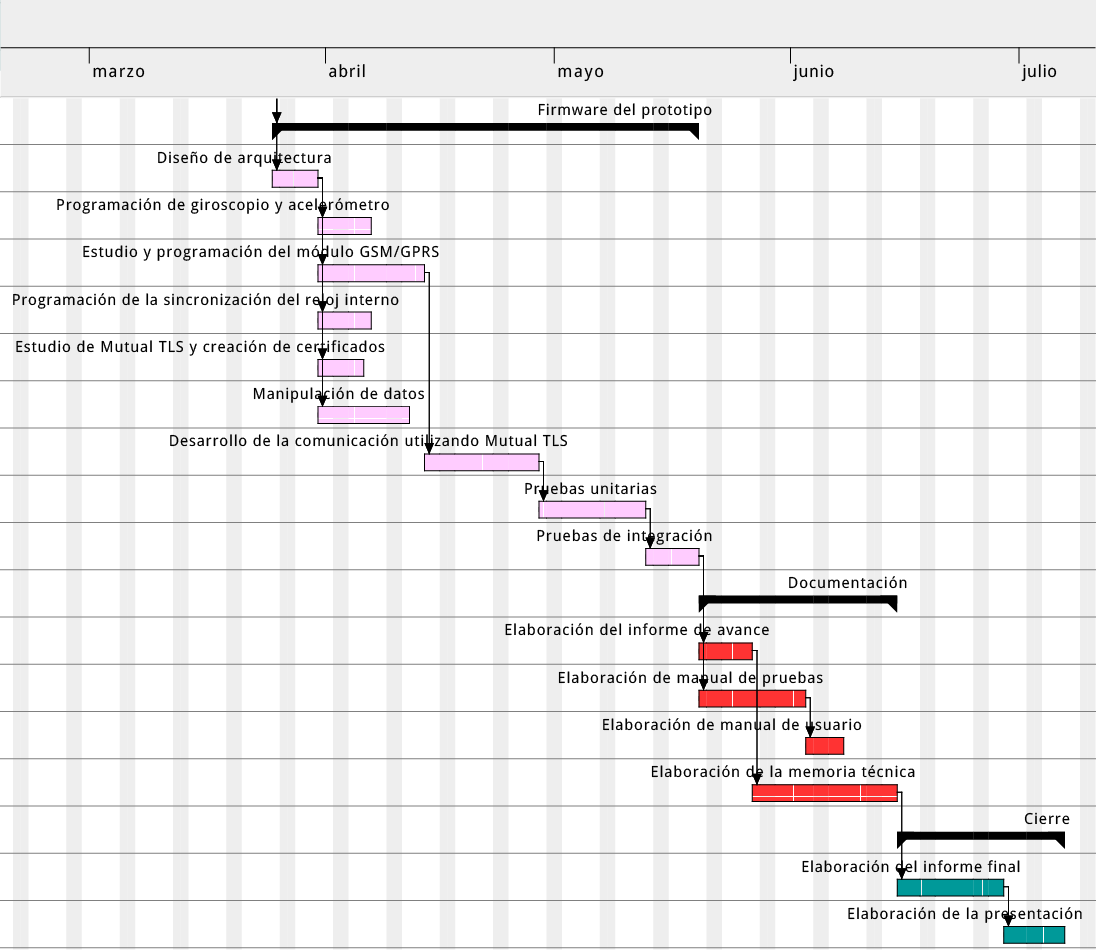
\includegraphics[width=1.1\textwidth]{./Figuras/gantt-4-bis.png}
\caption{Diagrama Gantt parte 4 de 4.}
\label{fig:gantt4}
\end{figure}

\section{12. Presupuesto detallado del proyecto}
\label{sec:presupuesto}

\begin{table}[htpb]
\centering
\begin{tabularx}{\linewidth}{@{}|X|c|r|r|@{}}
\hline
\rowcolor[HTML]{C0C0C0} 
\multicolumn{4}{|c|}{\cellcolor[HTML]{C0C0C0}COSTOS DIRECTOS} \\ \hline
\rowcolor[HTML]{C0C0C0} 
Descripción &
  \multicolumn{1}{c|}{\cellcolor[HTML]{C0C0C0}Cantidad} &
  \multicolumn{1}{c|}{\cellcolor[HTML]{C0C0C0}Valor unitario} &
  \multicolumn{1}{c|}{\cellcolor[HTML]{C0C0C0}Valor total} \\ \hline
 Horas desarrollo &
  \multicolumn{1}{c|}{640} &
  \multicolumn{1}{c|}{\$300,00} &
  \multicolumn{1}{c|}{\$192.000,00} \\ \hline
	Componentes electrónicos para un nodo&
  \multicolumn{1}{c|}{-} &
  \multicolumn{1}{c|}{\$2.307,00} &
  \multicolumn{1}{c|}{\$2.307,00} \\ \hline
\multicolumn{3}{|c|}{SUBTOTAL} &
  \multicolumn{1}{c|}{\$194.307,00} \\ \hline
\rowcolor[HTML]{C0C0C0} 
\multicolumn{4}{|c|}{\cellcolor[HTML]{C0C0C0}COSTOS INDIRECTOS} \\ \hline
\rowcolor[HTML]{C0C0C0} 
Descripción &
  \multicolumn{1}{c|}{\cellcolor[HTML]{C0C0C0}Cantidad} &
  \multicolumn{1}{c|}{\cellcolor[HTML]{C0C0C0}Valor unitario} &
  \multicolumn{1}{c|}{\cellcolor[HTML]{C0C0C0}Valor total} \\ \hline
	25\% del trabajo directo  &
  \multicolumn{1}{c|}{-} &
  \multicolumn{1}{c|}{-} &
  \multicolumn{1}{c|}{\$48.576,75} \\ \hline
\multicolumn{3}{|c|}{SUBTOTAL} &
  \multicolumn{1}{c|}{\$48.576,75} \\ \hline
\rowcolor[HTML]{C0C0C0}
\multicolumn{3}{|c|}{TOTAL} &
 \$242.883,75  \\ \hline
\end{tabularx}%
\end{table}

Detalle de componentes eletrónicos:
\begin{table}[htpb]
\centering
\begin{tabularx}{\linewidth}{@{}|X|c|r|r|@{}}
\hline
\multicolumn{4}{|c|}{\cellcolor[HTML]{C0C0C0}Componentes electrónicos para un nodo} \\ \hline
\rowcolor[HTML]{C0C0C0} 
Descripción &
  \multicolumn{1}{c|}{\cellcolor[HTML]{C0C0C0}Cantidad} &
  \multicolumn{1}{c|}{\cellcolor[HTML]{C0C0C0}Valor unitario} &
  \multicolumn{1}{c|}{\cellcolor[HTML]{C0C0C0}Valor total} \\ \hline
	Placa ESP32&
  \multicolumn{1}{c|}{1} &
  \multicolumn{1}{c|}{\$1.195,00} &
  \multicolumn{1}{c|}{\$1.195,00} \\ \hline
  	Sensor MPU6050 (giroscopio) &
  \multicolumn{1}{c|}{1} &
  \multicolumn{1}{c|}{\$283,00} &
  \multicolumn{1}{c|}{\$283,00} \\ \hline
	Sensor DHT11 (temperatura y humedad) &
  \multicolumn{1}{c|}{2} &
  \multicolumn{1}{c|}{\$140,00} &
  \multicolumn{1}{c|}{\$280,00} \\ \hline
	Sensor KY-037 (sonido)  &
  \multicolumn{1}{c|}{2} &
  \multicolumn{1}{c|}{\$175,00} &
  \multicolumn{1}{c|}{\$350,00} \\ \hline
	Modulo lector MicroSD  &
  \multicolumn{1}{c|}{1} &
  \multicolumn{1}{c|}{\$199,00} &
  \multicolumn{1}{c|}{\$199,00} \\ \hline

\multicolumn{3}{|c|}{SUBTOTAL} &
\multicolumn{1}{c|}{\$2.307,00} \\ \hline
\end{tabularx}%
\end{table}


\section{13. Gestión de riesgos}
\label{sec:riesgos}

A continuación se describirán los riesgos identificados para el desarrollo del proyecto.

\begin{itemize}[font=\bfseries]
	\item[a)] {\bf Identificación de los riesgos y estimación de sus consecuencias:}
	\begin{enumerate}
		\item La protección del prototipo contra la propolización no es adecuada.
\begin{itemize}
	\item[1.1] Severidad (S): 6, retrasa el proyecto ya que el funcionamiento del prototipo es afectado por la presencia de propóleos sobre su superficie.
	\item[1.2] Probabilidad de ocurrencia (O): 3, porque se extremarán las precauciones al cubrir el prototipo.
\end{itemize} 		
		\item La elección del microcontrolador no es correcta.
\begin{itemize}
	\item[2.1] Severidad (S): 4, porque la capacidad de recursos o de pines del micro seleccionado puede no ser suficiente para la solución. 
	\item[2.2] Probabilidad de ocurrencia (O): 2, se verificará que el producto seleccionado cubra todas las necesidades identificadas en el proyecto.
\end{itemize} 				
		\item La elección de los sensores no es correcta.
\begin{itemize}
	\item[3.1] Severidad (S): 4, si los sensores no cumplieran con lo que se requiere de ellos, o cualquier problema que hubiera para integrarlos al microcontrolador, se deberá investigar y adquirir nuevos.
	\item[3.2] Probabilidad de ocurrencia (O): 2, es baja ya que se analizará en detalle las especificaciones técnicas para evitar problemas.
\end{itemize} 				
		\item La calidad de los sensores no es buena.
\begin{itemize}
	\item[4.1] Severidad (S): 5, porque el rendimiento, comportamiento y fidelidad de los datos capturados deben ser aceptables para que el proyecto sea viable.
	\item[4.2] Probabilidad de ocurrencia (O): 4, porque la elección de los sensores está limitada a la oferta en el mercado y al presupuesto disponible.
\end{itemize} 				
		\item Falta de tiempo para completar el proyecto.
\begin{itemize}
	\item[5.1] Severidad (S): 5, si no se contara con el tiempo suficiente todas las tareas del proyecto se verian afectadas.
	\item[5.2] Probabilidad de ocurrencia (O): 5, la responsable es la única persona que trabajará en este proyecto, y sólo dispondrá de su tiempo libre para dedicárselo.
\end{itemize} 		
		\item No se dispone de una colmena para realizar pruebas.
\begin{itemize}
	\item[6.1] Severidad (S): 1, si no se contara con colmenas deberían incurrirse en tareas de simulación de la captura de mediciones.
	\item[6.2] Probabilidad de ocurrencia (O): 1, es baja ya que el cliente se ha comprometido a proveer de las colmenas necesarias.
\end{itemize} 			
	\end{enumerate}
	\item[b)] {\bf Tabla de gestión de riesgos:}

	\begin{table}[htpb]
	\centering
	\begin{tabularx}{\linewidth}{@{}|X|c|c|c|c|c|c|@{}}
	\hline
	\rowcolor[HTML]{C0C0C0} 
	Riesgo & S & O & RPN & S* & O* & RPN* \\ \hline
	La protección del prototipo contra la propolización no es adecuada       &  6 &  3 &  \cellcolor{red!25}18   &  2  &  1  &   \cellcolor{green!25}2   \\ \hline
	La elección del microcontrolador no es correcta       & 4  & 2  &  \cellcolor{green!25}8   &   - &  -  &    -  \\ \hline
	La elección de los sensores no es correcta       & 4  & 2  &  \cellcolor{green!25}8   &  -  &  -  &    -  \\ \hline
	La calidad de los sensores no es buena       & 5  & 4  &  \cellcolor{red!25}20   &  5  &  2  &   \cellcolor{green!25}10   \\ \hline
    Falta de tiempo para completar el proyecto &  5 & 5  &  \cellcolor{red!25}25   &  4  &  3  &    \cellcolor{green!25}12     \\ \hline
    No se dispone de una colmena para realizar pruebas & 1 & 1 & \cellcolor{green!25}1 & - & - & - \\ \hline
	\end{tabularx}%
	\end{table}
	
	Criterio adoptado: se tomarán medidas de mitigación en los riesgos cuyos números de RPN sean igual o mayor a 15.
	
	Nota: los valores marcados con (*) en la tabla corresponden luego de haber aplicado la mitigación.	
	
	\item[c)] {\bf Plan de mitigación de los riesgos que originalmente excedían el RPN máximo establecido:}
	
	A continuación se define el plan de mitigación para los riesgos 1, 4 y 5.
	
		\begin{enumerate}
			\item[1.] La protección del prototipo contra la propolización no es adecuada.
			\begin{itemize}
				\item Plan de mitigación: se instalará un componente electrónico de bajo costo dentro de la colmena, recubierto por la protección, previo a la instalación del prototipo.
				\item Severidad (S): 2, se pierde un componente que puede ser facilmente reemplazado.
				\item Probabilidad de Ocurrencia (O): 1, la ocurrencia de que falle la protección para el prototipo es muy baja.
			\end{itemize}
			\item[4.] La calidad de los sensores no es buena.
			\begin{itemize}
				\item Plan de mitigación: investigar en profundidad la oferta disponible en el mercado para realizar la mejor compra.
				\item Severidad (S): 5, se mantiene porque la calidad de los sensores es vital para la calidad y fiabilidad de las mediciones. 
				\item Probabilidad de Ocurrencia (O): 2, con más tiempo de análisis de la oferta se puede reduri la probabilidad de ocurrencia.
			\end{itemize}			
			\item[5.] Falta de tiempo para completar el proyecto.
			\begin{itemize}
				\item Plan de mitigación: solicitar días libres del trabajo para disponer de más tiempo.
				\item Severidad (S): 4, porque sigue siendo bloqueante no disponer de tiempo para dedicarle al proyecto. 
				\item Probabilidad de Ocurrencia (O): 3, porque es posible que el tiempo extra no alcance.
			\end{itemize}			
			
		\end{enumerate}
\end{itemize}

\section{14. Gestión de la calidad}
\label{sec:calidad}

A continuación se presentan los requerimientos con sus verificaciones y validaciones.

\begin{enumerate}
	\item Requerimientos del nodo de medición:
		\begin{enumerate}
			\item Deberá estar protegido para evitar que las abejas recubran su superficie con propóleo (propolización) que pueda afectar su funcionamiento.
				\begin{itemize}
					\item Verificación: se revisará que el prototipo esté completamente cubierto por el material seleccionado dentro de la colmena.
					\item Validación: se probará la eficacia del material que va a cubrir el prototipo dejando un elemento cubierto y comprobando que no presente rastros de propóleos en los días subsiguientes.
				\end{itemize}
			\item Deberá medir la temperatura en un rago de 0 \textdegree{}C--50 \textdegree{}C.
				\begin{itemize}
					\item Verificación: se verificará que el prototipo esté correctamente conectado con el sensor de temperatura y se adjuntará la hoja de datos del sensor.
					\item Validación: se hará una prueba con temperaturas dentro del rango estipulado y se contrastará las mediciones capturadas por el prototipo con un instrumento certificado.
				\end{itemize}			
			\item Deberá medir la humedad en un rango de 0--100\%.
				\begin{itemize}
					\item Verificación: se verificará que el prototipo esté correctamente conectado con el sensor de humedad y se adjuntará la hoja de datos del sensor.
					\item Validación: se hará una prueba simulando distintos niveles de humedad y se contrastará las mediciones capturadas por el prototipo con un instrumento certificado.
				\end{itemize}			
			\item Deberá medir el sonido en un rango de 100 Hz--10kHz.
				\begin{itemize}
					\item Verificación: se verificará que el prototipo esté correctamente conectado con el sensor de sonido y se adjuntará la hoja de datos del sensor.
					\item Validación: se hará una prueba con sonidos dentro del rango de frecuencias estipulado y se contrastará las mediciones capturadas por el prototipo con un instrumento certificado.
				\end{itemize}			
			\item Deberá medir la posición haciendo uso de un giroscopio y un acelerómetro.
				\begin{itemize}
					\item Verificación: se verificará que el prototipo esté correctamente conectado con el giroscopio y se adjuntará la hoja de datos del sensor.
					\item Validación: se hará una prueba con temperaturas dentro del rango estipulado y se contrastará las mediciones capturadas por el prototipo con un instrumento certificado.
				\end{itemize}		
			\item Deberá realizar las capturas cada 3 minutos.
				\begin{itemize}
					\item Verificación: se observará que se realicen las capturas cada 3 minutos.
					\item Validación: se dejará el prototipo corriendo y enviando mediciones a un backend mockeado donde se controlará que las mediciones hayan sido capturadas en intervalos de 3 minutos, independientemente de cuándo fueron recibidas.
				\end{itemize}			
			\item Deberá contar con tecnología GSM/GPRS para la conexión a la red de datos.
				\begin{itemize}
					\item Verificación: se verificará que el módulo GSM/GPRS esté incorporado en el prototipo y se incluirá la documentación técnica.
					\item Validación: se realizará una prueba de conexión a internet utilizando unicamente el módulo para comprobar que sea una solución suficiente para las necesidades del prototipo.
				\end{itemize}			
			\item Deberá tener un identificador unívoco.
			\item Deberá conectarse a un servidor externo para obtener la hora.
			\item Deberá sincronizar el reloj interno para que independientemente de la hora de impacto en el backend la hora de medición sea confiable.
				\begin{itemize}
					\item Verificación: se verificará que se haya incluido la lógica necesaria para conecarse a un servicio NTP.
					\item Validación: se contrastará la hora del prototipo con la hora real antes y después de conectarse al servicio NTP.
				\end{itemize}			
			\item Deberá contar con almacenamiento local (MicroSD).
				\begin{itemize}
					\item Verificación: se verificará que el prototipo esté correctamente conectado con el módulo de almacenamiento y se incluirá la hoja de datos del producto.
					\item Validación: se realizarán pruebas de almacenamiento comprobando luego desde un dispositivo externo que la información haya sido correctamente guardada en la microSD.
				\end{itemize}			
			\item Deberá tener capacidad para reintentar el envío de métricas ante pérdida de conexión.
				\begin{itemize}
					\item Verificación: se revisará que se haya implementado la lógica necesaria para el reintento de envío.
					\item Validación: se apagará la conexión a internet durante 10 minutos y al re-establecerse la conexión se deberá comprobar el envío de las médiciones pendientes.
				\end{itemize}			
		\end{enumerate}
	\item Requerimientos de seguridad:
		\begin{enumerate}
			\item Autenticación de los nodos y encriptación de los datos utilizando Mutual TLS.
				\begin{itemize}
					\item Verificación: se comprobará que se hayan generado los certificados necesarios y que estén desplegados tanto en el prototipo como en el backend.
					\item Validación: se habilitarán los logs en el backend para comprobar que la conexión con el prototipo se haya realizado de manera segura.
				\end{itemize}			
			\item Acceso a la aplicación web con usuario y contraseña.		
		\end{enumerate}
	\item Requerimientos de la aplicación backend:
		\begin{enumerate}
			\item Deberá enviar un alerta al usuario cuando detecte que la posición vertical de la colmena ha variado.		
			\item Deberá enviar un alerta al detectar que la temperatura en la cámara de cría varía por fuera de los 34\textdegree{}C--36\textdegree{}C.	
			\item Deberá enviar un alerta al usuario cuando detecte un cambio brusco de la temperatura en la cámara de cría.		
			\item Deberá emitir un alerta cuando se detecte que la humedad ha superado el 14\%.
				\begin{itemize}
					\item Verificación: se verificará que la lógica de definición de reglas, detección y envío de alertas haya sido desarrollada y probada.
					\item Validación: se simularán las condiciones que disparan las alertas y se comprobará que el usuario reciba las notificaciones.
				\end{itemize}			
			\item Deberá mantener un histórico de las métricas de hasta 2 años para comparar resultados de distintas temporadas.
	
		\end{enumerate}
	\item Requerimientos de la aplicación web:
		\begin{enumerate}		
			\item Deberá mostrar la temperatura en una serie temporal.	
			\item Deberá mostrar la humedad en una serie temporal.	
			\item Deberá mostrar el sonido en una serie temporal.		
			\item Deberá mostrar la posicion en una serie temporal.
				\begin{itemize}
					\item Verificación: se verificará que la lógica para la obtención y visualización de datos se encuentre desarrollada.
					\item Validación: se dispondrá de un set de mediciones de prueba para validar que los datos sean correctamente visualizados.
				\end{itemize}		
			\item Deberá mostrar la configuración personal del usuario.
				\begin{itemize}
					\item Verificación: se verificará que la lógica para la obtención, modificación y visualización de los datos personales del usuario haya sido implementada.
					\item Validación: se dispondrá de un usuario de prueba que se utilizará para validar el correcto funcionamiento del módulo.
				\end{itemize}			
			\item Deberá mostrar un histórico de los alertas.
				\begin{itemize}
					\item Verificación: se verificará que la lógica para la obtención y visualización de alertas se encuentre desarrollada.
					\item Validación: se dispondrá de un set de datos de alertas para validar que sean correctamente visualizados.
				\end{itemize}		
		\end{enumerate}
\end{enumerate}


\section{15. Procesos de cierre}    
\label{sec:cierre}

Las actividades asociadas al cierre estarán a cargo de la responsable del proyecto, Cynthia Escobar. \\
Se evaluará:
\begin{itemize}
	\item El grado de cumplimiento de los requerimientos originales. 
	\item Si hubo desvíos en el prepuesto y en los plazos estipulados.
	\item Si la arquitectura, las tecnologías y los sensores elegidos fueron los apropiados para la solución.
\end{itemize}
Los resultados del análisis previo serán registrados en la memoria.\\
Una vez finalizado el proyecto se procederá a realizar una reunión virtual para agradecer al cliente y a todos los colaboradores. También se incluirá un agradecimiento formal en la memoria.


\end{document}
